\documentclass[aspectratio=169]{beamer}

\usetheme{Madrid}
\usepackage[utf8]{inputenc}
\usepackage[T1]{fontenc}
\usepackage{lmodern}
\usepackage{amsmath,amssymb}
\usepackage{graphicx}
\usepackage{subcaption}
\usepackage{booktabs}
\usepackage{array}

\definecolor{ufrgsBlue}{RGB}{0,70,140}
\definecolor{ufrgsTeal}{RGB}{0,120,120}
\definecolor{ufrgsOrange}{RGB}{210,95,30}
\setbeamercolor{structure}{fg=ufrgsBlue}
\setbeamercolor{title}{fg=ufrgsBlue}
\setbeamercolor{frametitle}{fg=ufrgsBlue,bg=ufrgsBlue!8}
\setbeamertemplate{navigation symbols}{}
\setbeamertemplate{footline}[frame number]

\graphicspath{{../infufrgs/figures/}{../infufrgs/figures/equidistant/}}

\newcommand{\conceptplaceholder}[2]{%
    \begin{center}
    \setlength{\fboxsep}{10pt}%
    \fcolorbox{ufrgsOrange}{ufrgsOrange!8}{%
        \parbox{0.92\linewidth}{%
            \centering
            \textbf{Placeholder figure: #1}\\[0.4em]
            \small #2
        }%
    }%
    \end{center}
}

\title[Towards Local Interpretation]{Towards a Local Interpretation of Attention Based Neural Models}
\subtitle{PhD Thesis Proposal Presentation}
\author[B. W. S. R. Carvalho]{Breno W. Carvalho}
\institute[UFRGS]{Programa de Pos-Graduação em Computação \\ Universidade Federal do Rio Grande do Sul}
\date{March 2026}

\AtBeginSection[]{
    \begin{frame}{Roadmap}
        \tableofcontents[currentsection]
    \end{frame}
}

\begin{document}

\begin{frame}
    \titlepage
\end{frame}

\begin{frame}{Roadmap}
    \tableofcontents
\end{frame}

\section{Motivation and Questions}

\begin{frame}{Motivation}
    \begin{itemize}
        \item Attention-based models dominate language, vision, and multimodal benchmarks, but we still lack reliable local explanations for specific outputs.
        \item This proposal focuses on three connected fronts:
        \begin{itemize}
            \item emergence during training (grokking-like transitions),
            \item controllable neuro-symbolic steering,
            \item shift/attack diagnostics from internal features.
        \end{itemize}
        \item Core question: can we connect internal mechanisms to measurable, controllable behavior with explicit trade-offs?
    \end{itemize}
    \vspace{0.3em}
    \footnotesize References: \cite{vaswani2017attention,brown2020gpt3,openai2023gpt4,kautz2022thirdaisummer}
\end{frame}

\begin{frame}{Motivation: Why Local Explanations Matter}
    \small
    \begin{itemize}
        \item Current models perform well, but output quality alone does not explain \textit{why} a specific decision was produced.
        \item Without local explanations, we cannot reliably separate:
        \begin{itemize}
            \item real reasoning from spurious shortcuts,
            \item robust behavior from fragile behavior under shift,
            \item targeted control from collateral regressions.
        \end{itemize}
        \item The proposal therefore prioritizes measurable internal evidence, not only end-task scores.
    \end{itemize}
\end{frame}

\begin{frame}{Motivation: Emergence (G1)}
    \small
    \begin{block}{Question}
        How do useful internal structures emerge during training, especially around delayed generalization (grokking-like transitions)?
    \end{block}
    
    \begin{itemize}
        \item Analyze phase transitions in train/test behavior.
        \item Measure feature stability and cross-layer consistency around transition windows.
        \item Use controlled distribution shifts to stress-test emergence conditions.
    \end{itemize}
\end{frame}

\begin{frame}{Motivation: Neuro-symbolic Steering (G2)}
    \small
    \begin{block}{Question}
        Can we steer targeted behavior with logic constraints while keeping quality loss and collateral effects bounded?
    \end{block}
    \begin{itemize}
        \item Use sparse features and LTN validators as control signals.
        \item Compare constrained decoding against unconstrained and lightweight baselines.
        \item Report explicit quality-versus-satisfaction trade-offs.
    \end{itemize}
\end{frame}

\begin{frame}{Motivation: Diagnostics (G3)}
    \small
    \begin{block}{Question}
        Are internal sparse signatures better early-warning signals for shift/attacks than output-only heuristics?
    \end{block}
    \begin{itemize}
        \item Evaluate clean vs perturbed separation in latent space.
        \item Measure ROC-AUC, PR-AUC, calibration, and lead-time.
        \item Test transfer to settings where output confidence can be misleading.
    \end{itemize}
\end{frame}

\begin{frame}{Motivation Detail: Core Question in Operational Form}
    \small
    \begin{block}{Core question}
        Can we connect internal mechanisms to controllable behavior with explicit and reproducible trade-offs?
    \end{block}
    \vspace{0.4em}
    \begin{table}
        \centering
        \begin{tabular}{p{0.28\linewidth}p{0.62\linewidth}}
            \toprule
            \textbf{If yes, we should observe} & \textbf{How we verify} \\
            \midrule
            Stable local features & Cross-seed/epoch stability and reconstruction fidelity \\
            Targeted control & Constraint gain with bounded quality/regression cost \\
            Reliable diagnostics & Internal-signal performance at least matching output-only baselines \\
            \bottomrule
        \end{tabular}
    \end{table}
\end{frame}

\begin{frame}{Core Claims and Research Questions}
    \small
    \begin{table}
        \centering
        \begin{tabular}{p{0.18\linewidth}p{0.35\linewidth}p{0.38\linewidth}}
            \toprule
            \textbf{Claim} & \textbf{Research question} & \textbf{Hypothesis summary} \\
            \midrule
            C1: Emergence &
            Can controlled shifts induce delayed generalization with stable internal changes? &
            Late test gains align with increased cross-seed/cross-layer feature consistency. \\
            \addlinespace[0.3em]
            C2: Steering locality &
            Can logic constraints change targeted behavior with bounded regressions? &
            LTN-guided constraints improve rule satisfaction with acceptable quality loss. \\
            \addlinespace[0.3em]
            C3: Diagnostics &
            Are sparse internal signatures stronger than output-only heuristics for perturbation detection? &
            Sparse latent signatures improve or match detection/calibration stability. \\
            \bottomrule
        \end{tabular}
    \end{table}
\end{frame}

\begin{frame}{Proposal Positioning}
    \begin{columns}[T,onlytextwidth]
        \column{0.33\textwidth}
        \begin{block}{Completed}
            \footnotesize
            \begin{itemize}
                \item Controlled grokking evidence under distribution shift.
                \item Sparse SAE diagnostics for clean-vs-perturbed separation.
            \end{itemize}
        \end{block}
        \column{0.33\textwidth}
        \begin{block}{In Progress}
            \footnotesize
            \begin{itemize}
                \item Frozen steering protocol calibration.
                \item Final baseline and ablation matrix definition.
            \end{itemize}
        \end{block}
        \column{0.33\textwidth}
        \begin{block}{Pending}
            \footnotesize
            \begin{itemize}
                \item Final multi-seed runs and transfer/failure analysis.
                \item Thesis integration and defense-ready narrative.
            \end{itemize}
        \end{block}
    \end{columns}
\end{frame}

\section{Background and Objects}

\begin{frame}{Notation and Core Objects}
    \small
    \begin{itemize}
        \item Input sequence: $x_{1:T}$ and residual activations $h_{\ell}\in\mathbb{R}^{T\times d}$.
        \item Sparse representation at each layer: $s_{\ell}=E_{\ell}(h_{\ell})$, with decoder reconstruction $\hat{h}_{\ell}=D_{\ell}(s_{\ell})$.
        \item Cross-layer mapping: $T_{\ell\to k}(s_{\ell})\approx s_k$.
        \item Logic validators (LTN predicates/rules) output soft satisfaction scores in $[0,1]$.
    \end{itemize}
    \vspace{0.4em}
    \[
        S(Y_t)=\log P_{\mathrm{LM}}(Y_t)+w_{\mathrm{logic}}\cdot \mathrm{Sat}_{\mathrm{LTN}}(Y_t)
    \]
    \footnotesize
    This same object set is reused in G1 (emergence), G2 (steering), and G3 (diagnostics).
\end{frame}

\begin{frame}{Core Concepts Used in This Thesis}
    \small
    \begin{itemize}
        \item \textbf{Distributed representation:} useful concepts are encoded across multiple directions, so feature identity must be tested for stability.
        \item \textbf{Generalization dynamics:} delayed test gains require phase-aware analysis, not only endpoint metrics.
        \item \textbf{Optimization phases:} memorization and later reorganization can co-exist in the same run.
        \item \textbf{Practical implication:} C1/C2/C3 claims require paired behavioral + mechanistic evidence.
    \end{itemize}
\end{frame}

\begin{frame}{Transformer Internals Relevant to Interpretation}
    \small
    \begin{itemize}
        \item Attention acts as content-based routing:
        \[
            \mathrm{Attn}(Q,K,V)=\mathrm{softmax}\!\left(\frac{QK^\top}{\sqrt{d_k}}\right)V
        \]
        \item Residual stream is the main substrate for feature measurement:
        \[
            h_{\ell+1}=h_{\ell}+\Delta^{\text{attn}}_{\ell}(h_{\ell})+\Delta^{\text{mlp}}_{\ell}(h_{\ell})
        \]
        \item SAEs and transcoders operate over this layerwise residual interface.
    \end{itemize}
\end{frame}

\begin{frame}{Decoder Variants and Invariant Measurement Interface}
    \scriptsize
    \begin{table}
        \centering
        \setlength{\tabcolsep}{3pt}
        \begin{tabular}{@{}p{0.22\linewidth}p{0.26\linewidth}p{0.24\linewidth}p{0.23\linewidth}@{}}
            \toprule
            \textbf{Variant} & \textbf{Main change} & \textbf{Invariant object} & \textbf{Transfer risk} \\
            \midrule
            GPT-style dense decoder & Scale, data, recipe & $h_{\ell}$ and $s_{\ell}$ & Feature drift across checkpoints \\
            \addlinespace[0.2em]
            MoE decoder & Expert routing in FFN path & Residual hooks + validators & Route-dependent instability \\
            \addlinespace[0.2em]
            Long-context decoder & Context handling/efficiency & Same layerwise readout & Shifted activation statistics \\
            \addlinespace[0.2em]
            Instruction-aligned decoder & Objective / preference optimization & Same transcoder interface & Behavior shifts without clear internal causality \\
            \bottomrule
        \end{tabular}
        \setlength{\tabcolsep}{6pt}
    \end{table}
\end{frame}

\begin{frame}{Criteria for Actionable Mechanistic Interpretability}
    \small
    \begin{columns}[T,onlytextwidth]
        \column{0.49\textwidth}
        \begin{block}{Faithfulness and Stability}
            \begin{itemize}
                \item Internal measurements must track causal structure.
                \item Features should persist across seeds/checkpoints.
            \end{itemize}
        \end{block}
        \column{0.49\textwidth}
        \begin{block}{Transferability and Actionability}
            \begin{itemize}
                \item Features/validators should remain meaningful across layers.
                \item Explanations must support controllable interventions.
            \end{itemize}
        \end{block}
    \end{columns}
    \vspace{0.3em}
    \footnotesize
    In this proposal, these criteria are operationalized with reconstruction, sparsity, alignment, validator consistency, and steering-locality metrics.
\end{frame}

% \begin{frame}{Visual Concept Map}
%     \conceptplaceholder
%         {Unified architecture overview}
%         {Diagram to be added: token flow through model layers, SAE hooks per layer, cross-layer transcoder edges, and LTN validator heads feeding both analysis metrics and inference-time steering signals.}
%     \vspace{0.4em}
%     \footnotesize Placeholder created because this specific integrated diagram does not yet exist in \texttt{infufrgs/figures}.
% \end{frame}

\section{G1: Emergence and Grokking}

\begin{frame}{Grokking as Delayed Generalization}
    \begin{columns}[T,onlytextwidth]
        \column{0.56\textwidth}
        \begin{itemize}
            \item Grokking: test performance improves after training performance has already converged.
            \item Proposal claim: controlled train/test distribution shift is a strong inducer of this transition.
            \item Focus metric: transition delay and post-transition stability.
        \end{itemize}
        \footnotesize
        Key reference: \cite{carvalho2025inducing_grokking_distribution_shifts}
        \column{0.44\textwidth}
        \begin{figure}
            \centering
            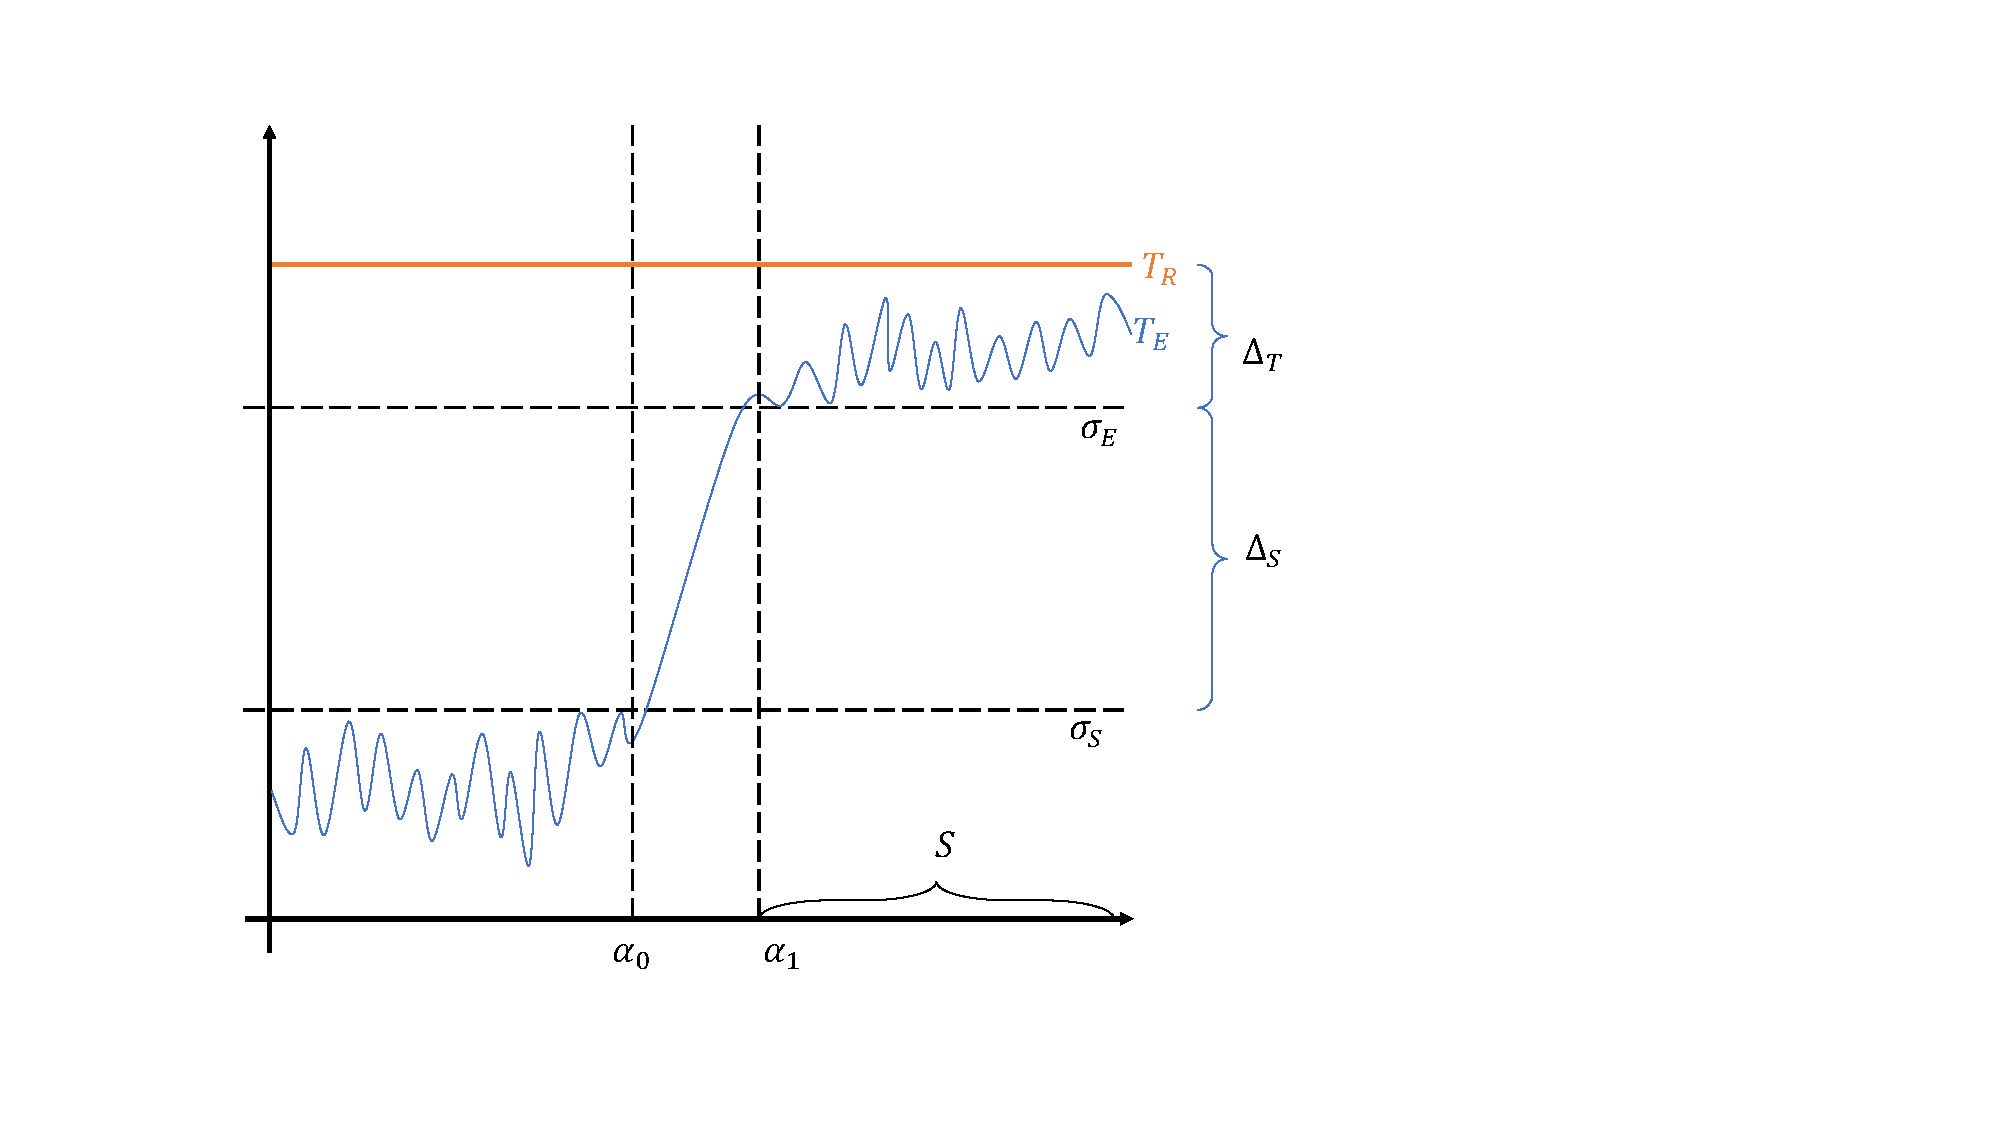
\includegraphics[width=\linewidth]{grokking_definition.pdf}
            \caption{Definition and phase regions used in this proposal.}
        \end{figure}
    \end{columns}
\end{frame}

\begin{frame}{Synthetic Datasets Used for Controlled Shift}
    \begin{columns}[T,onlytextwidth]
        \column{0.49\textwidth}
        \centering
        
\includegraphics[width=0.8\linewidth]{group_eqdist.pdf}
        
        {\scriptsize Equidistant subclasses}
        \column{0.49\textwidth}
        \centering
        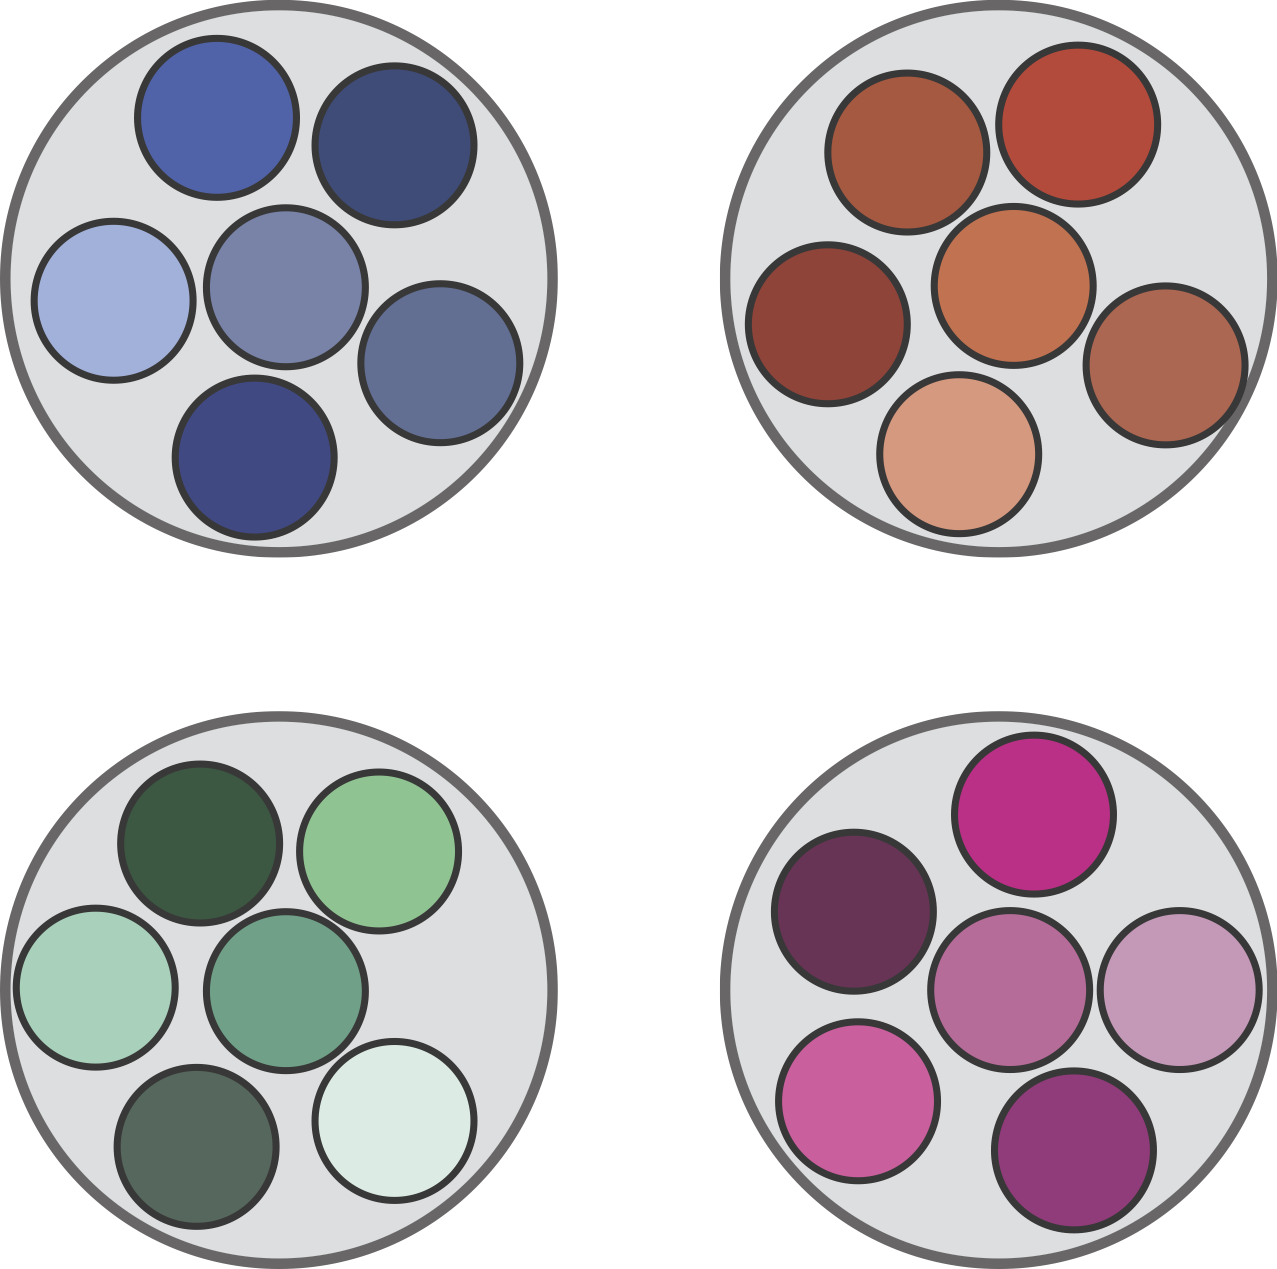
\includegraphics[width=0.64\linewidth]{group_eqvariant.png}
        
        {\scriptsize Equivariant subclasses}
    \end{columns}
    \small
    These datasets are designed to manipulate class/subclass coverage and isolate how shift structure impacts late generalization.
\end{frame}

\begin{frame}{Representative G1 Results}
    \begin{columns}[T,onlytextwidth]
        \column{0.49\textwidth}
        \begin{figure}
            \centering
            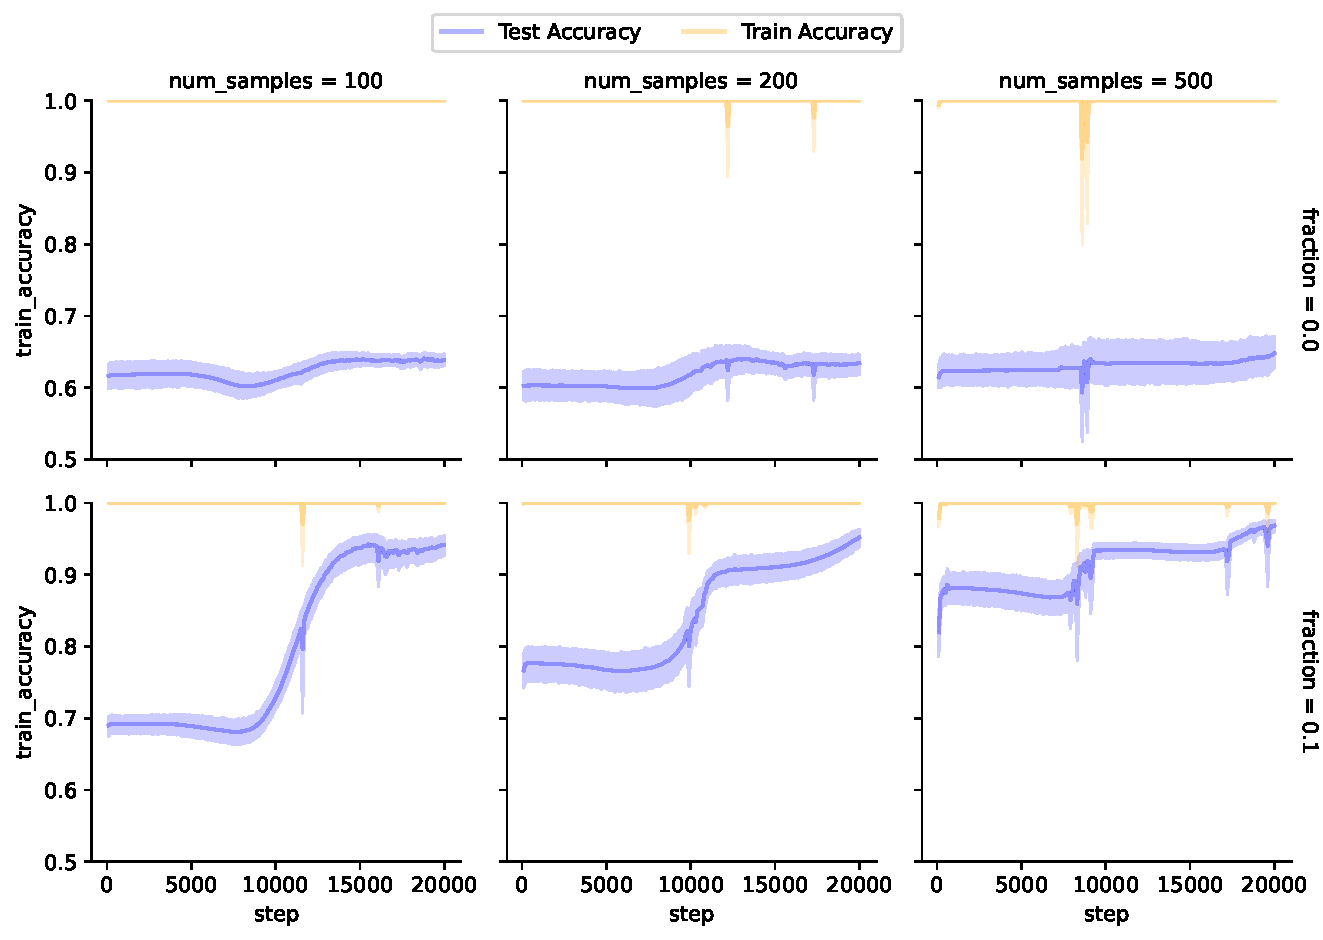
\includegraphics[width=\linewidth]{result_small.pdf}
            \caption{Small imbalance can induce late generalization.}
        \end{figure}
        \column{0.49\textwidth}
        \begin{figure}
            \centering
            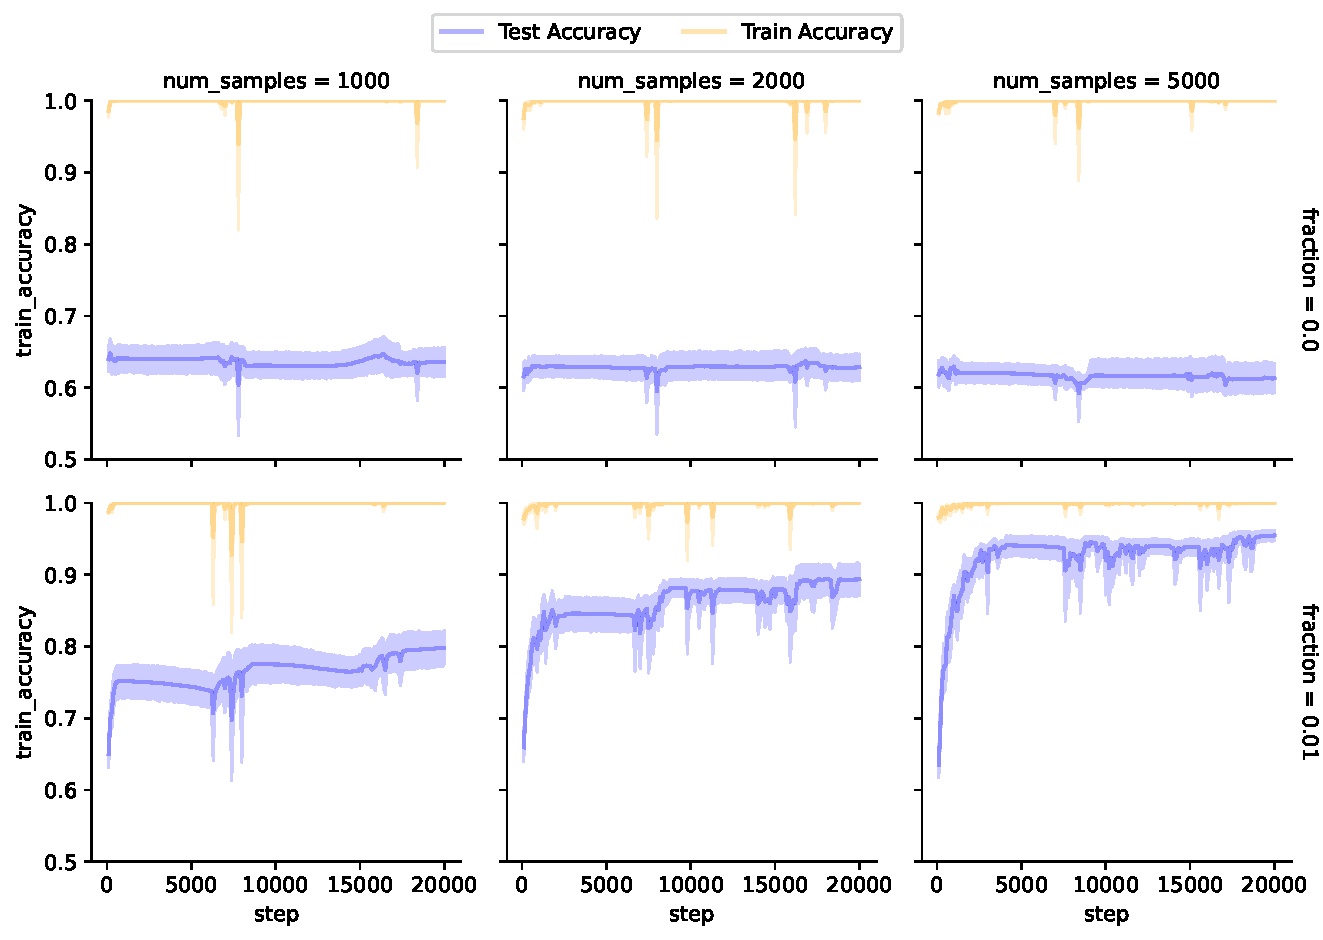
\includegraphics[width=\linewidth]{result_large.pdf}
            \caption{Shift-driven behavior remains visible at larger scale with strong imbalance.}
        \end{figure}
    \end{columns}
\end{frame}

\section{Methodology (G1-G3)}

\begin{frame}{LTN Cross-Layer Transcoder Pipeline}
    \begin{enumerate}
        \item Collect layerwise residual activations $h_\ell$.
        \item Train SAEs to obtain sparse codes $s_\ell$.
        \item Learn cross-layer mappings $T_{\ell\to k}$.
        \item Define LTN predicates/rules over sparse features.
        \item Use satisfaction scores for diagnostics and inference steering.
    \end{enumerate}
    % \vspace{0.6em}
    % \conceptplaceholder
    %     {Pipeline block diagram}
    %     {Figure to add: sequential pipeline from activations to sparse features to cross-layer alignment and logic scoring, with separate outputs for analysis metrics and decoding-time control.}
\end{frame}

\begin{frame}{Implementation Stages}
    \small
    \begin{table}
        \centering
        \begin{tabular}{p{0.18\linewidth}p{0.75\linewidth}}
            \toprule
            \textbf{Stage} & \textbf{Objective} \\
            \midrule
            1 & Reproducible setup: synthetic shift tasks, steering tasks, and perturbation suites. \\
            2 & Layerwise sparse feature learning with reconstruction/sparsity monitoring. \\
            3 & Cross-layer alignment with numeric and semantic consistency checks. \\
            4 & Logic-guided evaluation and steering with module ablations. \\
            5 & Multi-seed analysis, confidence intervals, reproducibility packaging. \\
            \bottomrule
        \end{tabular}
    \end{table}
\end{frame}

\begin{frame}{Evaluation Matrix}
    \tiny
    \begin{table}
        \centering
        \setlength{\tabcolsep}{2pt}
        \begin{tabular}{@{}p{0.15\linewidth}p{0.24\linewidth}p{0.29\linewidth}p{0.24\linewidth}@{}}
            \toprule
            \textbf{Goal} & \textbf{Tasks} & \textbf{Primary metrics} & \textbf{Baselines} \\
            \midrule
            G1 Emergence &
            Synthetic class/subclass shift settings &
            Delay-to-generalization, feature stability, cross-layer alignment &
            No-shift controls, dense probes \\
            \addlinespace[0.25em]
            G2 Steering locality &
            Single-rule and multi-rule constrained generation &
            Constraint satisfaction, quality, collateral regressions &
            Unconstrained, logit-bias only, rerank-only \\
            \addlinespace[0.25em]
            G3 Diagnostics &
            Clean vs stego and FGSM/PGD perturbations &
            ROC-AUC, PR-AUC, calibration, early-warning lead time &
            Output confidence or margin, dense detectors \\
            \bottomrule
        \end{tabular}
        \setlength{\tabcolsep}{6pt}
    \end{table}
\end{frame}

\section{Current Results}

\begin{frame}{What Is Already Demonstrated}
    \begin{block}{G1 feasibility}
        Controlled distribution-shift experiments repeatedly induce delayed generalization patterns and provide mechanism-discovery settings.
    \end{block}
    \begin{block}{G3 feasibility}
        Sparse-feature diagnostics separate clean and perturbed inputs with compact latent subsets.
    \end{block}
    \begin{block}{G2 status}
        Logic-guided steering architecture is implemented and validated at pilot level; frozen final matrix remains pending.
    \end{block}
    \footnotesize
    Evidence basis: \cite{carvalho2025inducing_grokking_distribution_shifts,carvalho2026interpretable_stego_detection_sae}
\end{frame}

\begin{frame}{G1 Effect Under Equivariant Shift}
    \begin{figure}
        \centering
        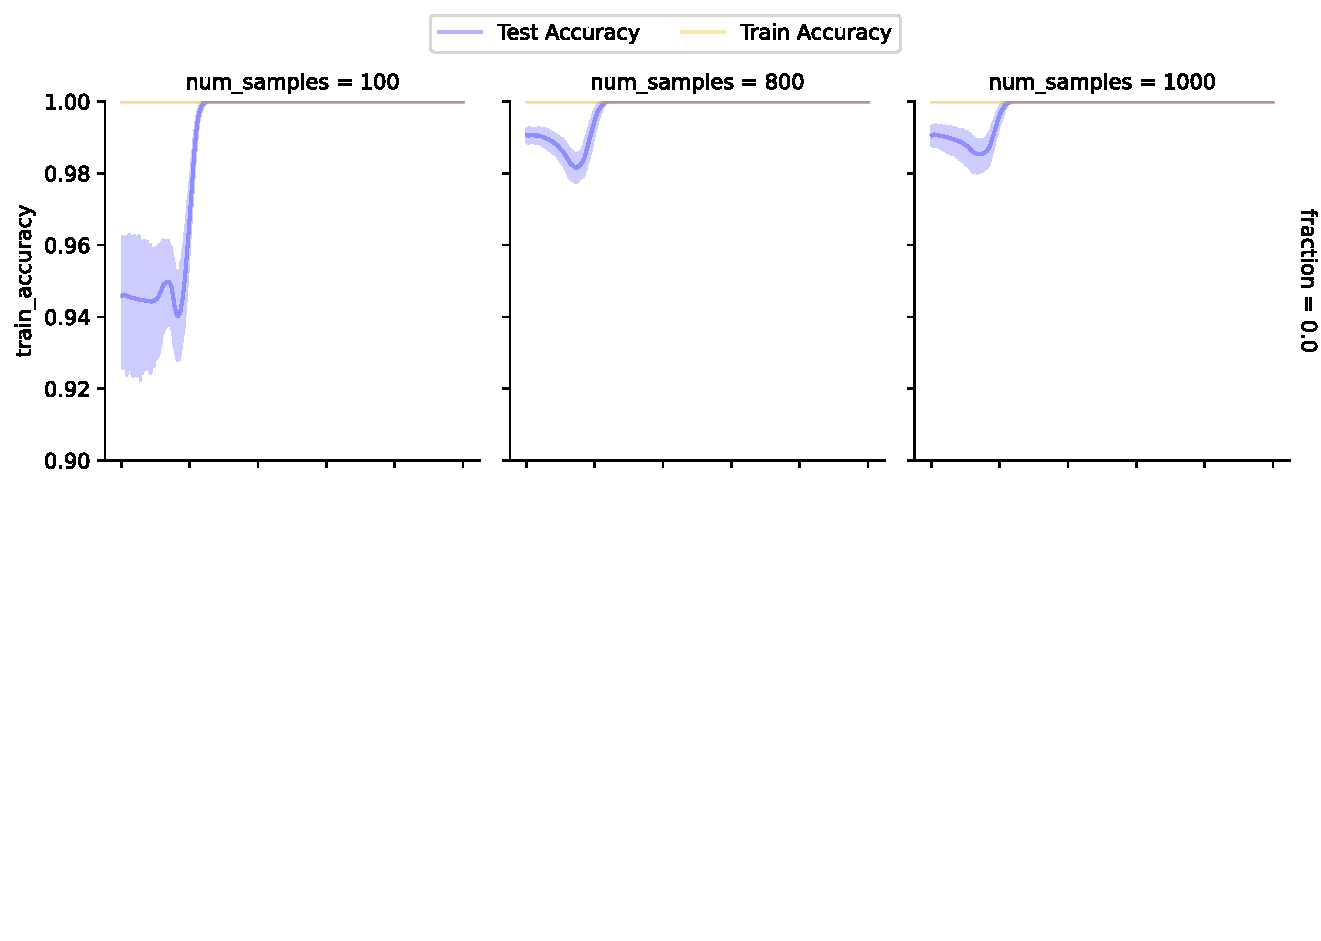
\includegraphics[width=0.75\linewidth]{result_exp_unb_samples_100_400_800_frac_0.0-1.0a.pdf}
        \caption{Representative behavior under equivariant subclass settings.}
    \end{figure}
\end{frame}

% \begin{frame}{Steering Evidence to Add in Final Runs}
%     \conceptplaceholder
%         {Logic-guided decoding loop}
%         {Figure to add: stepwise beam-search diagram showing candidate expansion, predicate grounding with LoRA adapters, LTN satisfaction scoring, reranking by composite score, and pruning to the next beam.}
%     \vspace{0.5em}
%     \small
%     This placeholder marks the visual that should summarize the frozen G2 protocol and latency/quality trade-off points.
% \end{frame}

\section{Timetable}

\begin{frame}{Status Windows (as of February 2026)}
    \scriptsize
    \begin{table}
        \centering
        \begin{tabular}{p{0.2\linewidth}p{0.35\linewidth}p{0.35\linewidth}}
            \toprule
            \textbf{Window} & \textbf{Thesis writing and structure} & \textbf{Experiments and analysis} \\
            \midrule
            Completed by Jan 31, 2026 &
            Chapter 2 baseline revision; Chapter 4 structure and evaluation matrix drafted; sections 4.2--4.4 drafted. &
            Steering pipeline prototypes implemented; single/multi-rule setup configured; reproducibility scaffold initiated. \\
            \addlinespace[0.25em]
            In progress (February 2026) &
            Revise Chapter 4 with advisor feedback; consolidate proposal-facing manuscript; consistency checks and committee-ready version. &
            Run pending ablations (no LTN / no $T_{\ell\to k}$ / sparsity variants); calibrate validators; freeze steering protocol. \\
            \addlinespace[0.25em]
            Planned (March-April 2026) &
            Incorporate final feedback; freeze defense manuscript; submit final committee version and post-defense corrections. &
            Freeze final results/figures; complete reproducibility checks; defense rehearsals and defense execution. \\
            \bottomrule
        \end{tabular}
    \end{table}
\end{frame}

\begin{frame}{Completed Items vs Remaining Items}
    \small
    \begin{columns}[T,onlytextwidth]
        \column{0.49\textwidth}
        \begin{block}{Completed}
            \begin{itemize}
                \item Research direction and scope are clearly defined.
                \item Full conference paper accepted (A3+ target track).
                \item Core grokking experiments and analyses consolidated.
                \item Preliminary logic-based steering experiments available.
            \end{itemize}
        \end{block}
        \column{0.49\textwidth}
        \begin{block}{To be completed}
            \begin{itemize}
                \item Submit full journal paper (A3+ requirement track).
                \item Consolidate final steering method and definitive experiments.
                \item Finalize all thesis chapters and full integration.
                \item Complete administrative steps, defense, and corrections.
            \end{itemize}
        \end{block}
    \end{columns}
\end{frame}

\section{Conclusion and Future Work}

\begin{frame}{Conclusion}
    \begin{itemize}
        \item The proposal unifies emergence analysis, neuro-symbolic steering, and perturbation diagnostics in one local-interpretability program.
        \item The methodology jointly measures sparse feature geometry, cross-layer consistency, and logic satisfaction.
        \item Current evidence already supports feasibility for G1 and G3; G2 is positioned for final protocol-level validation.
    \end{itemize}
    \vspace{0.5em}
    \small
    Expected outcome: a practical, testable local analysis and intervention framework with explicit trade-offs and uncertainty reporting.
\end{frame}

\begin{frame}{Expected Contributions and Future Work}
    \small
    \begin{enumerate}
        \item Unified local-interpretability pipeline (SAE + $T_{\ell\to k}$ + LTN validators).
        \item Empirical evidence on emergence dynamics under controlled shifts.
        \item Measurable steering-locality framework with quality-vs-satisfaction curves.
        \item Transferable sparse diagnostics for perturbation/shift detection.
    \end{enumerate}
    \vspace{0.4em}
    \begin{block}{Immediate future work}
        Finalize frozen G2 runs, complete ablations and transfer tests, integrate results in final manuscript, and prepare defense-ready reproducibility artifacts.
    \end{block}
\end{frame}

\begin{frame}{Main Risks and Mitigations}
    \small
    \begin{table}
        \centering
        \begin{tabular}{@{}p{0.16\linewidth}p{0.34\linewidth}p{0.42\linewidth}@{}}
            \toprule
            \textbf{Risk} & \textbf{Impact} & \textbf{Mitigation} \\
            \midrule
            R1: Sparse feature instability &
            Weak reproducibility of local explanations &
            Multi-seed protocols, feature matching across runs, confidence intervals. \\
            \addlinespace[0.25em]
            R2: Weak semantic alignment across layers &
            Numeric fit without meaningful transfer &
            Validator-consistency checks and identity/baseline ablations. \\
            \addlinespace[0.25em]
            R3: Constraint gains with excessive quality loss &
            Steering not practical for deployment &
            Rule-weight calibration, Pareto reporting, unconstrained fallback baseline. \\
            \addlinespace[0.25em]
            R5: Time pressure near defense &
            Reduced ablation coverage &
            Freeze minimum publishable matrix and defer non-critical extensions. \\
            \bottomrule
        \end{tabular}
    \end{table}
\end{frame}

\section*{References}

\begin{frame}[allowframebreaks]{References}
    \bibliographystyle{alpha}
    \bibliography{../infufrgs/biblio,../infufrgs/biblio-grokking}
\end{frame}


\end{document}
